% theroy syntethic images
Synthetic images are computer-generated visuals that replicate real-world scenes or objects. They are increasingly used in computer vision when collecting real-world data is either difficult, expensive, or raises privacy concerns. These images are especially useful for training machine learning models for tasks like object detection, image classification, and scene reconstruction. By generating synthetic data, developers can create tailored datasets that meet specific needs, which is crucial for industries like healthcare, self-driving cars, and surveillance, where real-world data may be hard to gather. \cite{jimaging8110310}

\section{Advantages of Synthetic Data for CV Models}

Synthetic data is very helpful in computer vision, especially when collecting real-world data is expensive, limited, or difficult. Deep learning models need a lot of data to work well, and when these models evolve, the need for large datasets keeps growing. \cite{10.1145/3042064, nikolenko2021synthetic} This creates challenges for areas like medical imaging, face recognition, surveillance, and self-driving cars, where getting real-world data is often hard, time-consuming, or even impossible. \cite{10.1007/978-3-642-15549-9_55} Synthetic data provides a way to solve these challenges by offering a reliable alternative to real-world data.

\subsection{Customization}
One of the key benefits of synthetic data is customization. Synthetic images allow developers to create and change environments to meet specific needs. A scene can include various objects, environments, and camera setups, all of which can be adjusted to match the requirements of a particular application. \cite{jimaging8110310, rajpura2017objectdetectionusingdeep} Customization provides possibilities to generate diverse and complex scenes, and recreate scenarios that would be difficult or impossible to capture in the real world. This ability to design scenes to match an environment removes the need to rely on real-world data collection. The dataset can then contain the exact conditions and variations needed to train a model effectively. 

\subsection{Ethics}
Another big benefit is ethics. Synthetic data solves privacy problems because it doesn’t use real people’s information. For example, in face recognition tasks, using synthetic faces eliminates the need to collect photos of real people, avoiding privacy concerns and consent issues. Similarly, in medical applications, synthetic data can replace real patient data, protecting privacy while still providing useful training material for AI systems . This is especially important in healthcare, where patient confidentiality is critical, and real-world datasets may be small or hard to share across organizations. \cite{jimaging8110310}

\subsection{Randomization}
Randomization builds upon the scalability of synthetic data by introducing variety into the dataset. It is important for creating a robust dataset, as it ensures the model is trained on diverse scenarios rather than a single, repetitive situation.\cite{borkman2021unityperceptiongeneratesynthetic} A dataset full of similar images of the same scene won’t help a model generalize well and may lead to overfitting. Overfitting occurs when a model performs well on training data but struggles to generalize to new, unseen data. \cite{Ying_2019} Randomization helps prevent this issue by introducing small, controlled variations in the data, making the model more adaptable and better equipped to handle real-world variability.

Compared to manually collecting real images, randomization allows for the creation of an almost unlimited variety of scenarios in a fraction of the time. With real-world data, obtaining different perspectives or environmental conditions might require extensive setup or access to rare situations, making synthetic data and randomization more efficient and scalable. \cite{borkman2021unityperceptiongeneratesynthetic}

With synthetic data, randomization can be applied in many ways. It can be used to randomly change the objects in a scene through transformations, such as rotations, scaling, or color. The background and environment can also be changed, including lighting, weather, or the scene’s layout. Additionally, randomization can be applied to the camera settings, such as adjusting the position, tilt, or angle, to generate a variety of perspectives. \cite{borkman2021unityperceptiongeneratesynthetic}

This flexibility allows for the automatic generation of unlimited, diverse training data without manually altering each scene. Randomization scripts make it easier and faster to create a wide range of scenarios, increasing the robustness of the computer vision model.

Further details on the implementation of randomization in synthetic data generation will be explained in the Theory: Unity, and Method chapters.


\section{Image Labeling}

Image labeling is essential in computer vision because it gives machine learning models the information they need to understand and interpret visual data. Without labeled images, a model wouldn’t know what is right or wrong and couldn’t learn correctly. \cite{Labelling}

Labeling involves creating another image or annotation that defines where the object is located in the original training image. It works like an answer, giving the model the correct outputs to aim for during training. During training, the model is given both the images and their labels. The model compares its predictions with the labeled data and makes adjustments to improve its accuracy. Over time, through iteration, the model learns how to correctly identify and classify objects in new images based on the labeled examples. \cite{Labelling}

\subsection{Labeling Methods}

There are different ways to label objects in images, depending on the level of detail needed. Two common methods are bounding boxes and segmentation.

Bounding boxes use rectangles to highlight the location of objects, providing a simple and effective way to represent their positions. This method works well for tasks requiring only rough localization but does not capture precise shapes or boundaries.

Segmentation in computer vision assigns a label to each pixel in an image, effectively separating objects from their surroundings. This method provides detailed boundary information by dividing an image into regions, often visualized with unique colors or patterns for different objects or areas. Unlike bounding boxes, segmentation captures the exact shape and spatial details of objects, offering a pixel-level understanding of the image. \cite{labelingMethods}

\begin{figure}[H]
    \centering
    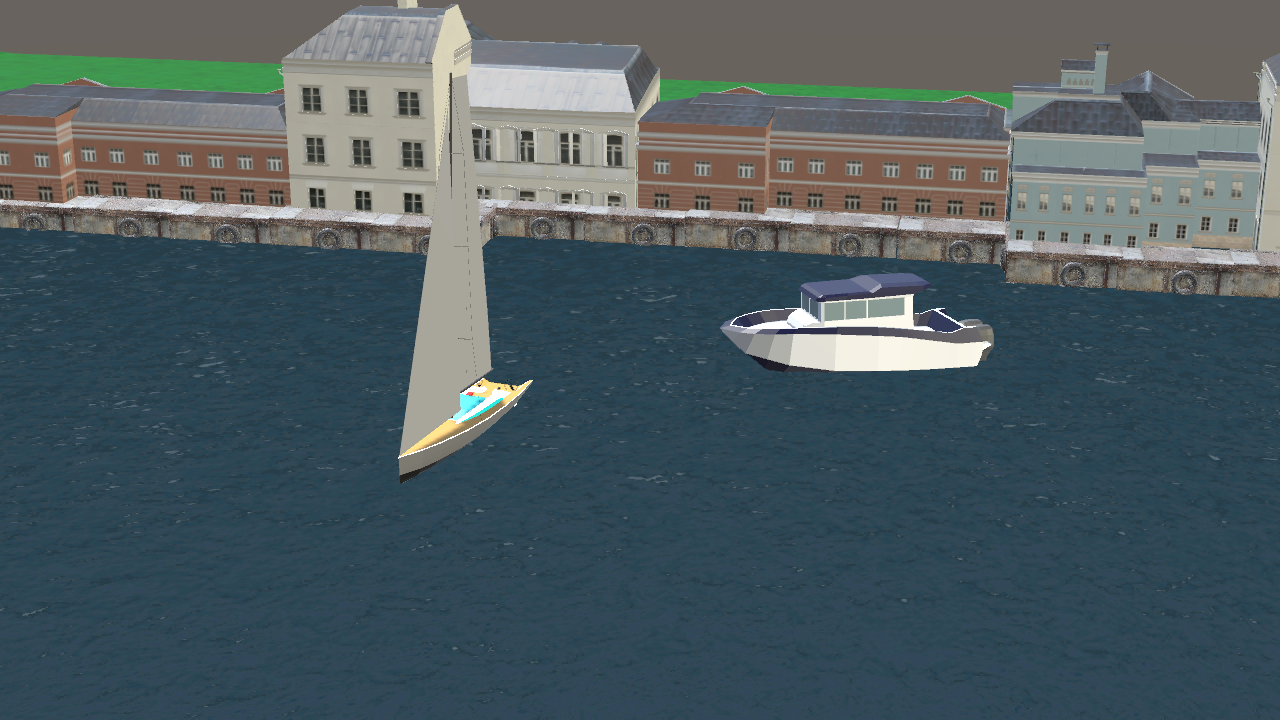
\includegraphics[width=0.7\textwidth]{Figures/rgb_2.png}
    \caption{Original image}
    \label{fig:image1}
\end{figure}

\begin{figure}[H]
    \centering
    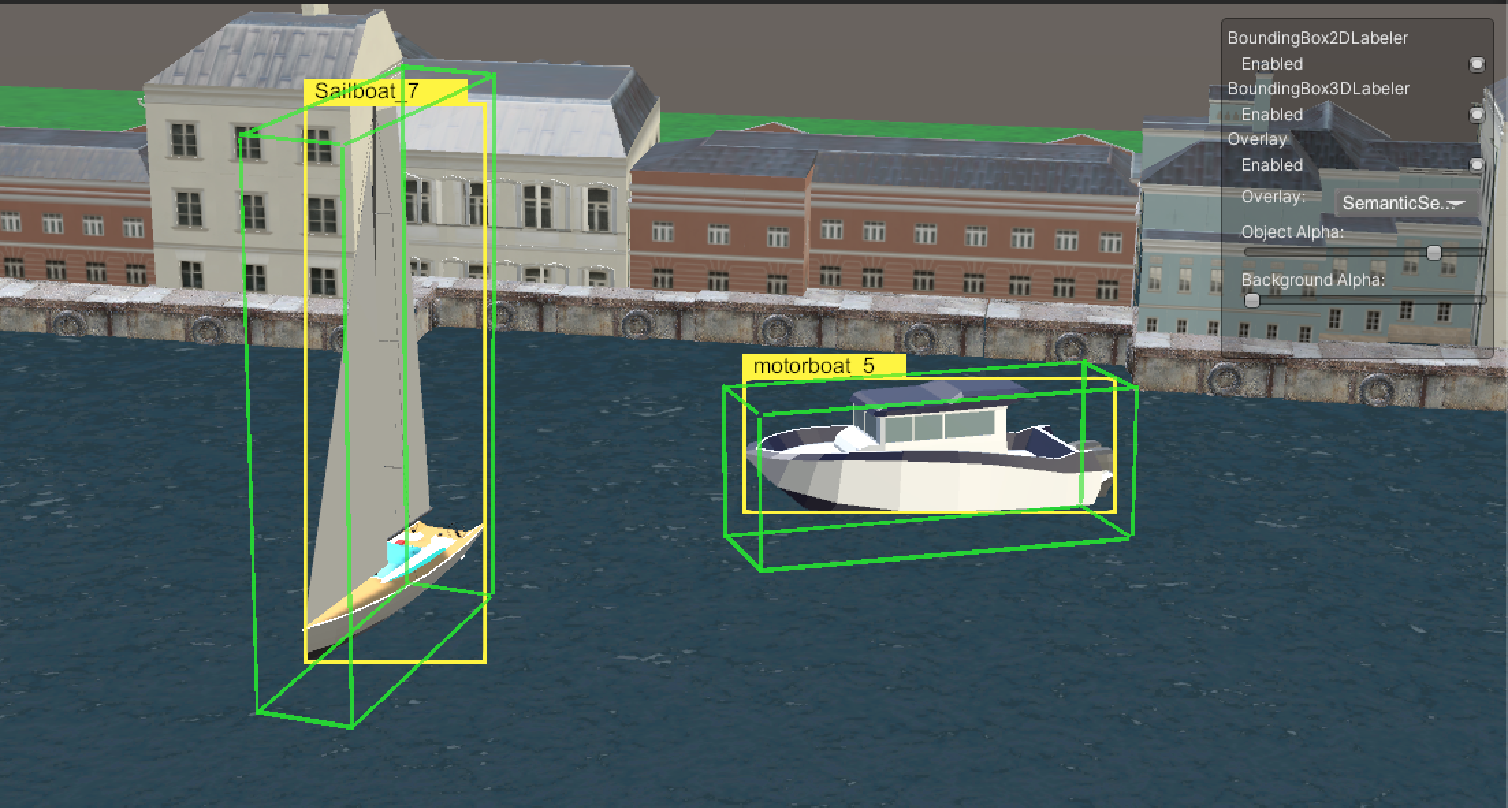
\includegraphics[width=0.7\textwidth]{Figures/boundingbox.png}
    \caption{Bounding boxes}
    \label{fig:image2}
\end{figure}

\begin{figure}[H]
    \centering
    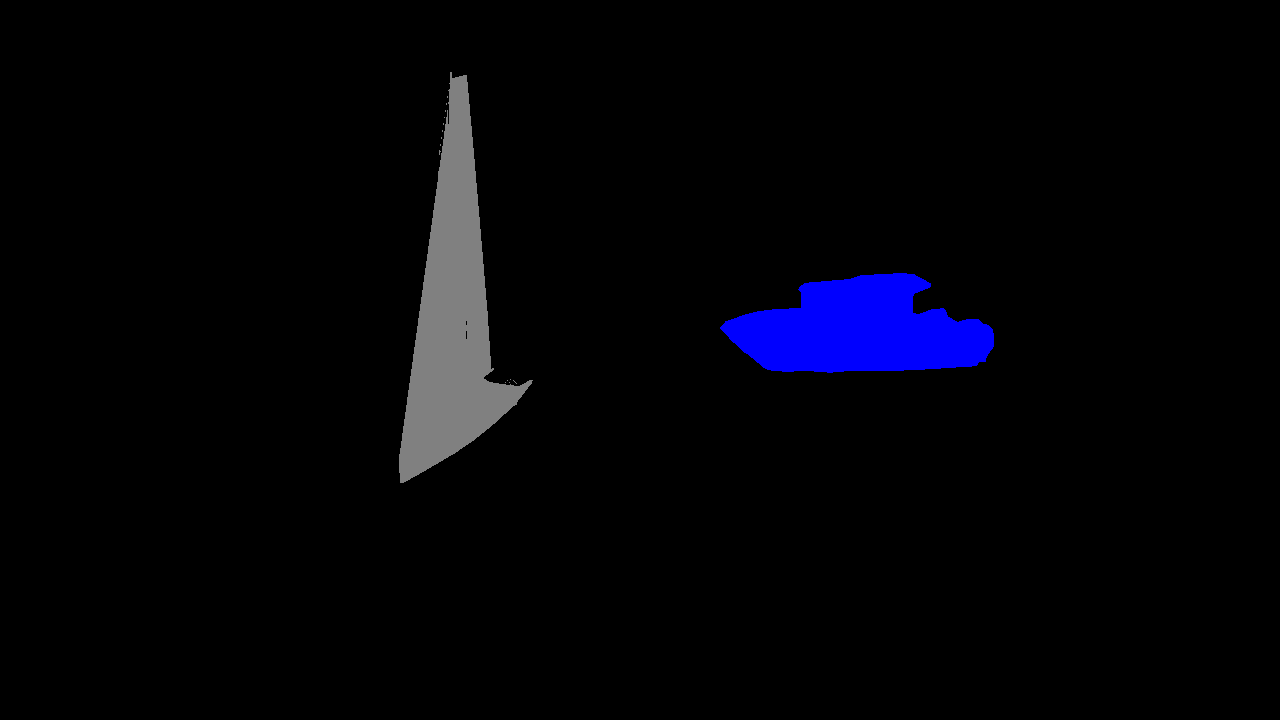
\includegraphics[width=0.7\textwidth]{Figures/segmentation_2.png}
    \caption{Segmentation}
    \label{fig:image3}
\end{figure}




\subsection{Advantages with Synthetic Labeling}
Labeling is a major benefit of working with synthetic data. Using real images requires manual effort for labeling, which involves identifying and annotating each object in the dataset. As dataset sizes grow, manual labeling becomes increasingly impractical. Annotating thousands of real-world images needs significant human labor and can include inconsistencies, potentially impacting model accuracy and robustness negatively. \cite{nikolenko2021synthetic}

In contrast, synthetic images provide the advantage of automatic labeling during generation through the rendering pipeline. Platforms like Unity, offer automated labeling capabilities via the Perception Package. \cite{unity-perception2022} This ensures pixel-perfect annotations, including bounding boxes and segmentation masks, with no manual intervention. The automated process delivers consistent, high-quality annotations for every image while saving considerable time and effort.


\section{Balancing Realism in Synthetic Data}
While synthetic image generation offers numerous benefits for computer vision models, a key challenge is achieving sufficient realism. The domain gap between synthetic and real-world data can significantly impact model performance.\cite{nikolenko2021synthetic}  Although it is possible to create highly realistic scenes, some aspects remain particularly difficult to simulate. For instance, dynamic surfaces like water in maritime applications can be a challenge due to its complex behavior with reflections and refractions. \cite{waterrendering} Similarly, obtaining realistic 3D renderings of objects like boats and other maritime structures can be difficult.

Going for a realistic synthetic datasets can also be expensive and time consuming and may outweigh the benefits, especially when high realism is unnecessary for certain tasks. Instead, specific optimizations and techniques like domain adaptation can help bridge the gap between synthetic and real-world data. \cite{nikolenko2021synthetic, jimaging8110310} By balancing realism and practicality, synthetic datasets can achieve a level that meets the needs of specific applications without excessive computational costs.


\section{The Future of Image Generation}

Using AI to generate images for computer vision models has become an increasingly powerful tool, with Generative Adversarial Networks (GANs) being a popular in this field. GANs consist of two neural networks that work in a competitive process to create realistic synthetic data. The generator produces fake data, while the discriminator evaluates whether the data is real or fake, with both networks improving through this competition. This dynamic has made GANs highly effective for tasks like image generation, domain adaptation, and creating privacy-preserving synthetic datasets. Despite their potential, training GANs can be challenging due to issues like instability and the risk of producing data with limited diversity. These challenges can hinder the model’s ability to generalize and innovate. \cite{gan} GANs and other AI-driven innovations are helping reduce the time and cost of creating datasets, while also enabling the simulation of complex scenarios and environments. However, using AI to train AI introduces additional risks such as overfitting and hallucination, where models generate outputs that are not only inaccurate but may also be entirely fictional or irrelevant. Hallucinations often arise from poor-quality training data that the model may overfit during training, leading to distorted results. Tackling this challenge requires the development of new techniques to detect and correct these errors, ensuring more reliable and trustworthy synthetic data. \cite{hallucination}
